% h = 4.135667696923859e-15
% Frequenz g, o, b, v: [5.49000051e+14 5.19607006e+14 6.87865585e+14 7.35181858e+14]
\nocite{anleitungV500}
\section{Auswertung}
\label{sec:Auswertung}

\subsection{Strom-Spannungs Kennlinie und Beleuchtungsstärke}
Die gemessenen Photoströme und die zugehörigen Spannungen bei vollsändiger Beleuchtungsstärke sind in der Tabelle (\ref{tab:Strom-Spannung}) aufgelistet. 
Zusätzlich sind die Photströme bei einer halben Beleuchtungsstärke in der Tabelle (\ref{tab:halbe-Stärke}) aufgeführt.
Für die Auswertung werden allerdings diese und die folgenden Spannungen der Messungen mit (-1) multipliziert, damit für die Berechnung der Planck-Konstante 
das richtige Vorzeichen herauskommt. Jedoch wird durch das wechselnde Vorzeichen der Spannungen die weitere Auswertung qualitativ nicht benachteiligt. Diese
Umrechnung wäre durch umschalten des Schaltbilds nicht nötig gewesen. \\
Mithilfe der beiden Messreihen werden zwei Strom-Spannungs Kennlinien in der Abbildung (\ref{fig:Plot1}) graphisch dargestellt. Der Verlauf dieser beiden
Messreihen entspricht den Erwartungen. Bei einer höheren Beschleunigungsspannung nähert sich der Photostrom asymptotisch den Maximum an. Wenn die Spannung sich
der Grenzspannung annähert, nimmt der Photostrom quadratitisch ab. Dieser Verlauf wird in der Abbildung (\ref{fig:blau}) genauer dargestellt. Außerdem ist anhand der Abbildung (\ref{fig:Plot1})
zu erkennen, dass der Photostrom sich mit einem kleinem Spalt bzw. mit einer kleineren Belecuhtungsstärke, ebenfalls verkleinert. 
\begin{figure}[H]
    \centering
    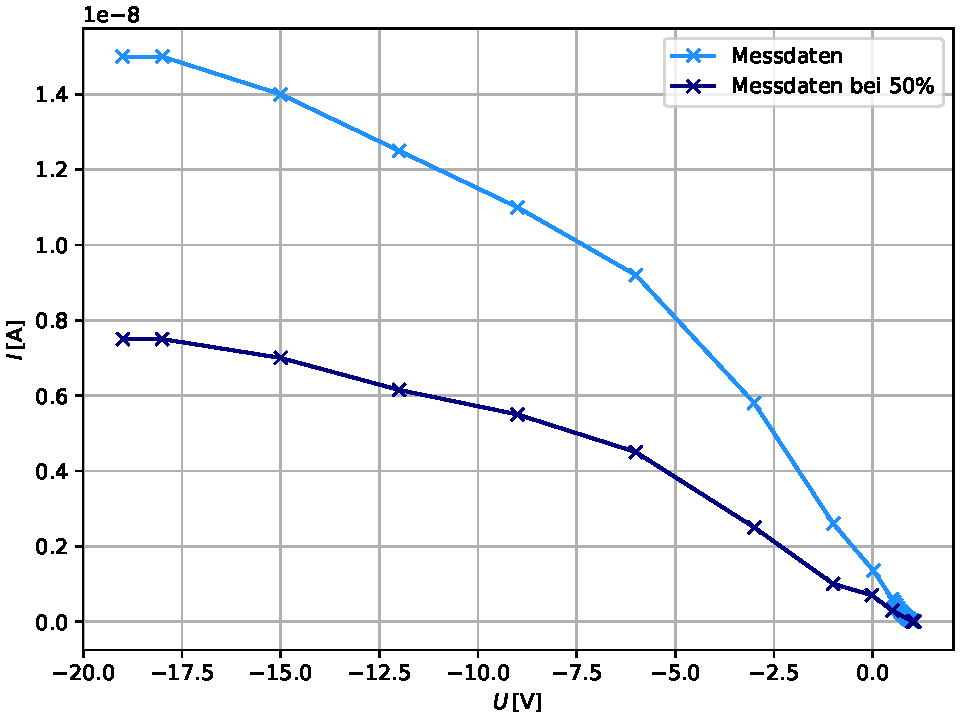
\includegraphics[width=0.8\textwidth]{Plots/Plot1.pdf}
    \caption{Strom-Spannungs Kennlinien der blauen Linien bei zwei verschiedenen Beleuchtungsstärken.}
    \label{fig:Plot1}
\end{figure}
\begin{table}[H]
    \centering
    \caption{Gemessene Photoströme in Abhängigkeit der Spannung bei ganzer Beleuchtungsstärke.}
    \label{tab:Strom-Spannung}
    \begin{tblr}{colspec ={c c || c c || c c}}
        \toprule
        $U\,[\unit{\volt}]$ & $I\,[\unit{\nano\ampere}]$ & $U\,[\unit{\volt}]$ & $I\,[\unit{\nano\ampere}]$ & $U\,[\unit{\volt}]$ & $I\,[\unit{\nano\ampere}]$\\
        \midrule
        -1,05   & 0     & -0,80   & 0,160 & -0,02   & 1,350\\
        -1,00   & 0,030 & -0,78   & 0,175 & 1,00    & 2,600\\
        -0,96   & 0,038 & -0,76   & 0,200 & 3,00    & 5,800\\
        -0,94   & 0,052 & -0,74   & 0,230 & 6,00    & 9,200\\
        -0,92   & 0,062 & -0,72   & 0,255 & 9,00    & 11,00\\
        -0,90   & 0,078 & -0,70   & 0,280 & 12,00   & 12,50\\
        -0,88   & 0,090 & -0,65   & 0,360 & 15,00   & 14,00\\
        -0,86   & 0,105 & -0,60   & 0,440 & 18,00   & 15,00\\
        -0,84   & 0,115 & -0,55   & 0,520 & 19,00   & 15,00\\
        -0,82   & 0,140 & -0,50   & 0,600 &  & \\
        \bottomrule
    \end{tblr}
\end{table}
\begin{table}[H]
    \centering
    \caption{Gemessene Photoströme in Abhängigkeit der Spannung bei halber Beleuchtungsstärke.}
    \label{tab:halbe-Stärke}
    \begin{tblr}{colspec ={c c || c c }}
        \toprule
        $U\,[\unit{\volt}]$ & $I\,[\unit{\nano\ampere}]$ & $U\,[\unit{\volt}]$ & $I\,[\unit{\nano\ampere}]$\\
        \midrule
        19,00      & 7,50   & 3,00       & 2,50 \\
        18,00      & 7,50   & 1,00       & 1,00 \\
        15,00      & 7,00   & 0,02       & 0,70 \\
        12,00      & 6,15   & -0,50      & 0,29 \\
        9,00       & 5,50   & -1,00      & 0,07 \\
        6,00       & 4,50   & -1,05      & 0    \\  
        \bottomrule
    \end{tblr}
\end{table}

\subsection{Grenzspannungen für verschiedene Wellenlängen}
\label{sec:Grenzspannungen}
In den Abbildungen (\ref{fig:violet}), (\ref{fig:blau}), (\ref{fig:gruen}) und (\ref{fig:orange}) sind die Messdaten des linearen Verlaufs
des Photostroms für verschiedene Wellenlängen dargestellt. Hierfür ist $\sqrt{I}$ gegen $U$ aufgetragen und es wird jeweils eine Ausgleichsgerade
eingezeichnet. Mithile dieser Abbildungen lassen sich die verschiedenen Grenzspannungen in Abhängigkeit der Wellenlänge bestimmen. Die zugehörigen Messdaten
sind in den Tabellen (\ref{tab:violet}), (\ref{tab:Strom-Spannung}), (\ref{tab:gruen}) und (\ref{tab:orange}) aufgelistet.\\
Die Ausgleichsgeraden entsprechen der From $$\sqrt{I} = m \cdot U + b\,.$$ Daraus ergibt sich für die Grenzspannung $$U_{\text{G}} = \frac{-b}{m}\,.$$
Demnach ergeben sich die folgenden Grenzspannungen 
\begin{align*}
    U_{\text{G, violett}} &= (1,21\pm0,15)\,\unit{\volt}\\
    U_{\text{G, blau}} &= (1,09\pm0,10)\,\unit{\volt}\\
    U_{\text{G, grün}} &= (0,62\pm0,07)\,\unit{\volt}\\
    U_{\text{G, orange}} &= (0,54\pm0,04)\,\unit{\volt}\,.\\
\end{align*}

\begin{figure}[H]
    \centering
    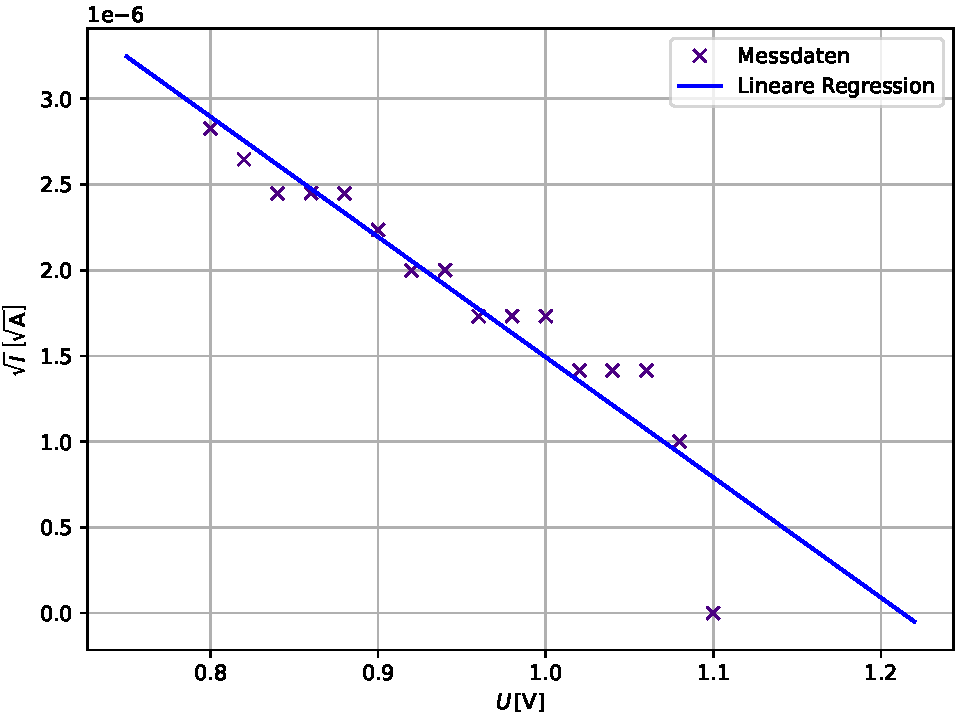
\includegraphics[width=0.8\textwidth]{Plots/violet.pdf}
    \caption{Graphische Darstellung der Messreihe und Ausgleichsgerade für die violette Linie.}
    \label{fig:violet}
\end{figure}
\begin{figure}[H]
    \centering
    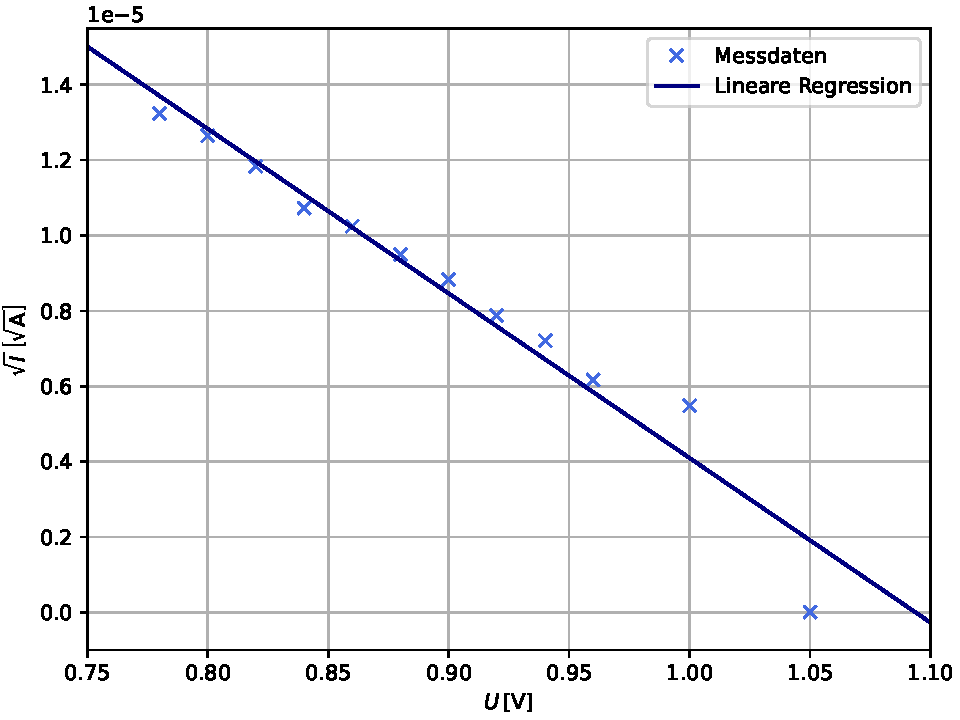
\includegraphics[width=0.8\textwidth]{Plots/blau.pdf}
    \caption{Graphische Darstellung der Messreihe und Ausgleichsgerade für die blaue Linie.}
    \label{fig:blau}
\end{figure}
\begin{figure}[H]
    \centering
    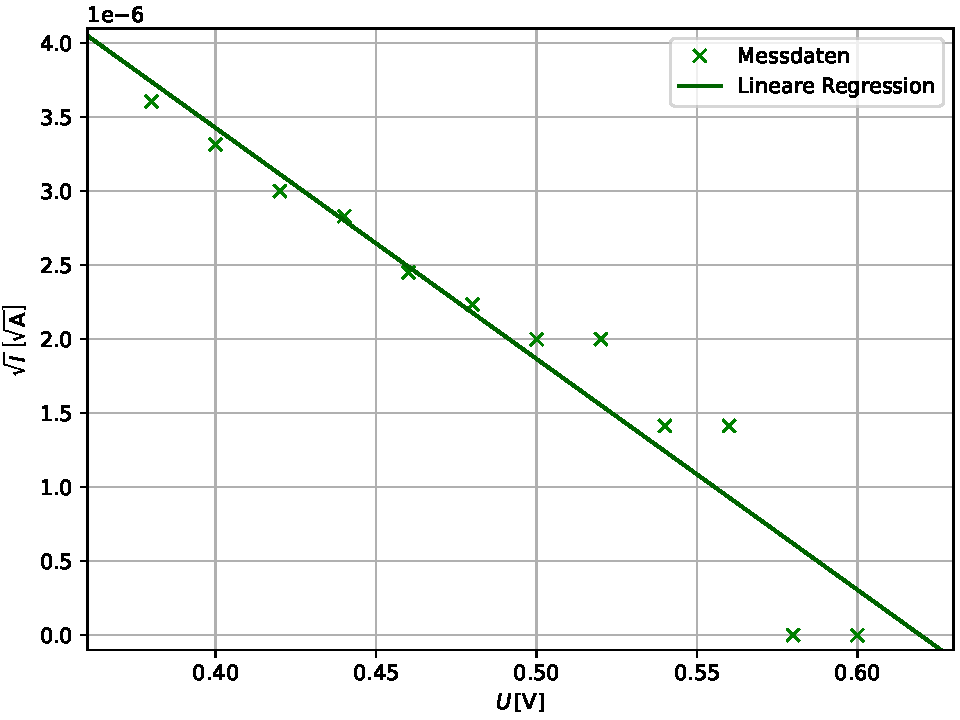
\includegraphics[width=0.8\textwidth]{Plots/gruen.pdf}
    \caption{Graphische Darstellung der Messreihe und Ausgleichsgerade für die grüne Linie.}
    \label{fig:gruen}
\end{figure}
\begin{figure}[H]
    \centering
    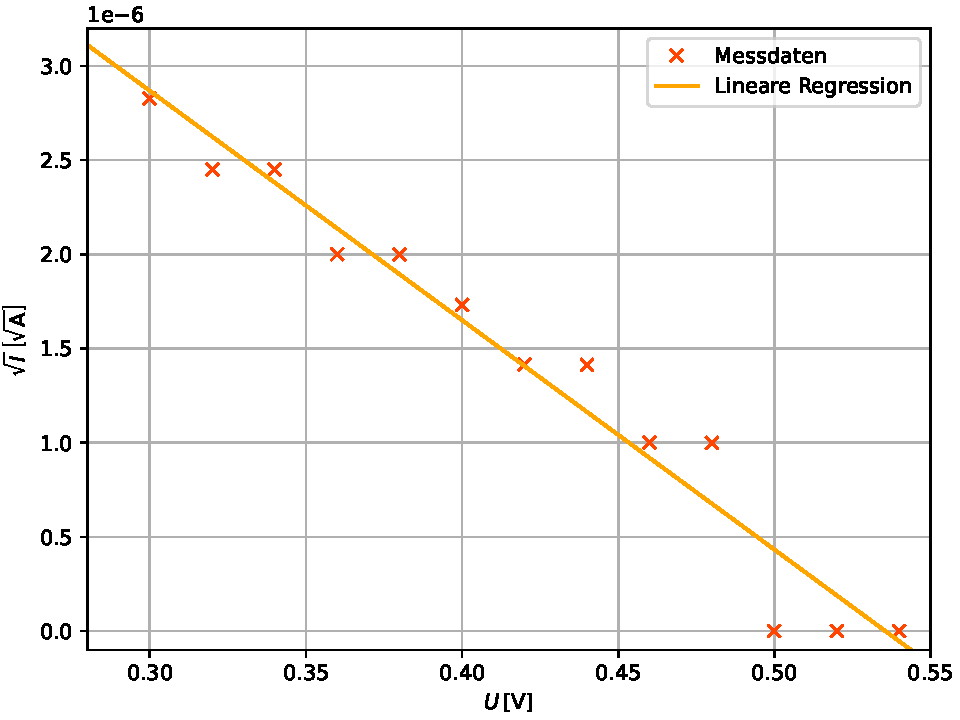
\includegraphics[width=0.8\textwidth]{Plots/orange.pdf}
    \caption{Graphische Darstellung der Messreihe und Ausgleichsgerade für die orangene Linie.}
    \label{fig:orange}
\end{figure}

\begin{table}[H]
    \centering
    \caption{Gemessene Photoströme in Abhängigkeit der Spannung für die violette Linie.}
    \label{tab:violet}
    \begin{tblr}{colspec ={c c || c c }}
        \toprule
        $U\,[\unit{\volt}]$ & $I\,[\unit{\pico\ampere}]$ & $U\,[\unit{\volt}]$ & $I\,[\unit{\pico\ampere}]$\\
        \midrule
        -1.10   & 0 & -0.94   & 4 \\
        -1.08   & 1 & -0.92   & 4 \\
        -1.06   & 2 & -0.90   & 5 \\
        -1.04   & 2 & -0.88   & 6 \\
        -1.02   & 2 & -0.86   & 6 \\
        -1.00   & 3 & -0.84   & 6 \\
        -0.98   & 3 & -0.82   & 7 \\
        -0.96   & 3 & -0.80   & 8 \\
        \bottomrule
    \end{tblr}
\end{table}
\begin{table}[H]
    \centering
    \caption{Gemessene Photoströme in Abhängigkeit der Spannung für die grüne Linie.}
    \label{tab:gruen}
    \begin{tblr}{colspec ={c c || c c }}
        \toprule
        $U\,[\unit{\volt}]$ & $I\,[\unit{\pico\ampere}]$ & $U\,[\unit{\volt}]$ & $I\,[\unit{\pico\ampere}]$\\
        \midrule
        -0.6        & 0 & -0.48       & 5 \\
        -0.58       & 0 & -0.46       & 6 \\
        -0.56       & 2 & -0.44       & 8 \\
        -0.54       & 2 & -0.42       & 9 \\
        -0.52       & 4 & -0.40       & 11 \\
        -0.50       & 4 & -0.38       & 13 \\
        \bottomrule
    \end{tblr}
\end{table}
\begin{table}[H]
    \centering
    \caption{Gemessene Photoströme in Abhängigkeit der Spannung für die orangene Linie.}
    \label{tab:orange}
    \begin{tblr}{colspec ={c c || c c }}
        \toprule
        $U\,[\unit{\volt}]$ & $I\,[\unit{\pico\ampere}]$ & $U\,[\unit{\volt}]$ & $I\,[\unit{\pico\ampere}]$\\
        \midrule
        -0.54   & 0 & -0.40   & 3 \\
        -0.52   & 0 & -0.38   & 4 \\
        -0.50   & 0 & -0.36   & 4 \\
        -0.48   & 1 & -0.34   & 6 \\
        -0.46   & 1 & -0.32   & 6 \\
        -0.44   & 2 & -0.30   & 8 \\
        -0.42   & 2 & & \\
        \bottomrule
    \end{tblr}
\end{table}

\subsection{Planck-Konstante und Austrittsarbeit des Kathodenmaterials}
Um die Plank-Konstante und die Austrittsarbeit zu bestimmen, werden die Grenzspannungen benötigt.
Zunächst werden die Grenzspannungen betrachtet, welche anhand der jeweiligen Tabellen abgelesen werden. 
Diese werden anschließend gegen die Frequenz $f$ aufgetragen und eine Ausgleichsgerade wird eingezeichnet.
Die zugehörigen Frequenzen sind in der Tabelle (\ref{tab:Wellenlaengen}) aufgeführt.
Die Ausgleichsgerade ergibt sich aus den Gleichungen (\ref{eqn:}) und (\ref{eqn:}), weswegen die Steigung der Planck-Konstante in 
\unit{\eV\second} und der Betrag vom $y$-Achsen Abschnitt der Austrittsarbeit $\phi_{\text{A}}$ in \unit{\eV} entspricht. Daraus folgt
\begin{align*}
    h_{\text{exp,}1} &= (2,95 \pm 0,25)\,\unit{\eV\second}\\
    \phi_{\text{A,exp,}1} &= (1,03 \pm 0,16) \, \unit{\eV}\,.\\
\end{align*}
\begin{figure}[H]
    \centering
    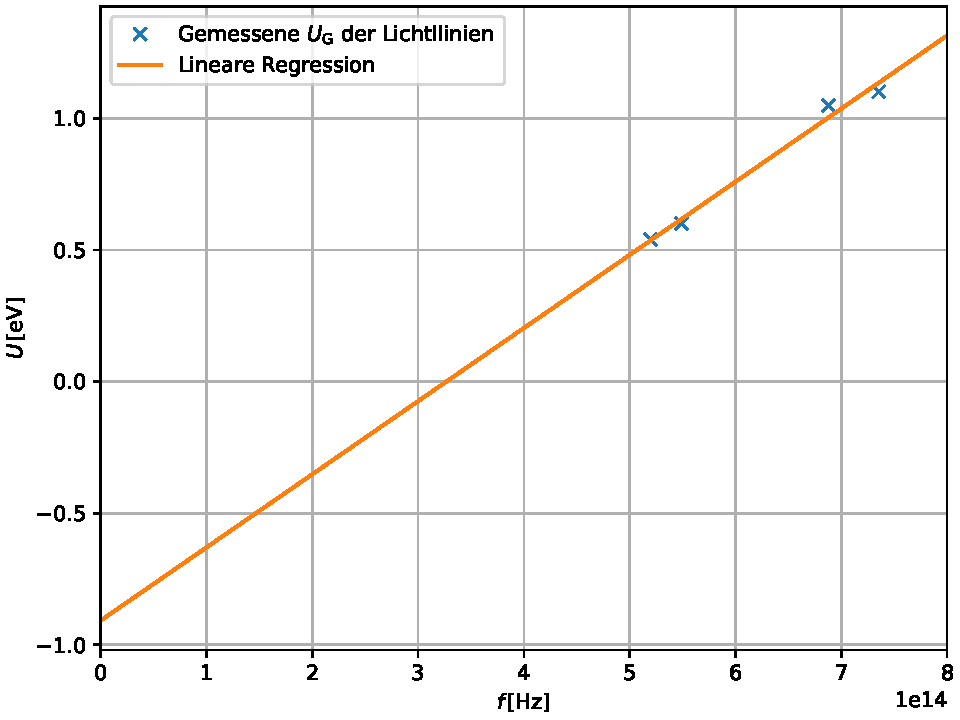
\includegraphics[width=0.8\textwidth]{Plots/planck_gemessen.pdf}
    \caption{Gemessene Grenzspannungen in Abhängigkeit der Frequenz mit einer Ausgleichsgerade.}
    \label{fig:Planck_gemessen}
\end{figure}
Bei der zweiten Methode wird die Planck-Konstante sowie die Austrittsarbeit mithilfe der berechneten Grenzspannungen
aus den Ausgelichsgeraden in (\ref{sec:Grenzspannungen}) berechnnet. Damit werden wie bei der ersten Methode die Grenzspannungen
gegen die Frequenz aufgetragen und eine Ausgleichsgerade durchgezogen. Durch die Ausgleichsgerade ergeben sich die Werte 
\begin{align*}
    h_{\text{exp,}2} &= (3,219 \pm 0,098)\,\unit{\eV\second}\\
    \phi_{\text{A,exp,}2} &= (1,14 \pm 0,06) \, \unit{\eV}\,.\\
\end{align*}
\begin{figure}[H]
    \centering
    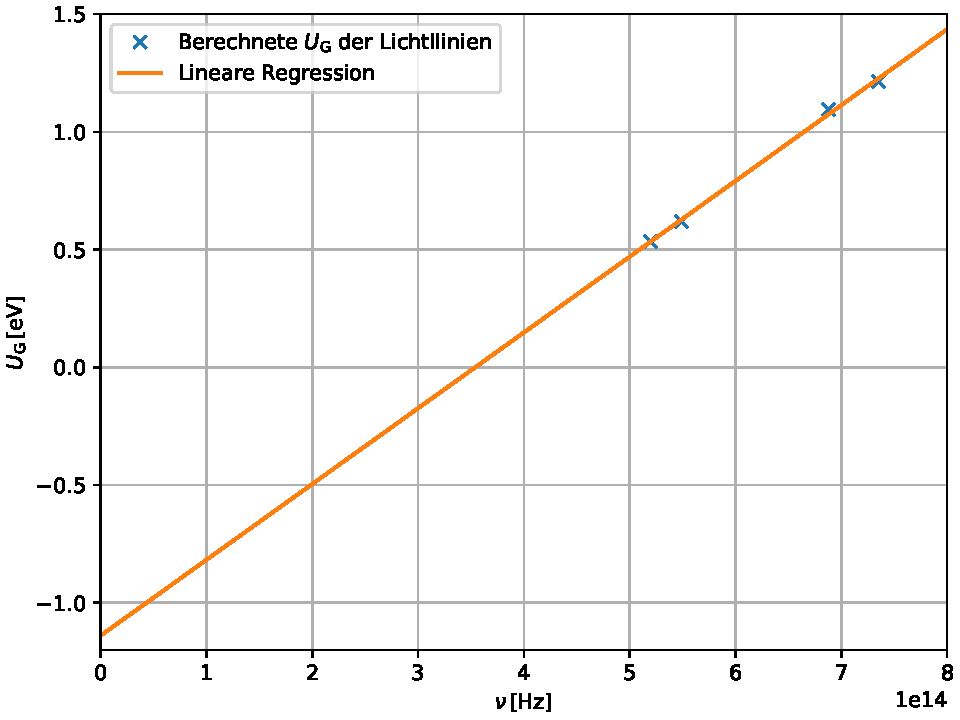
\includegraphics[width=0.8\textwidth]{Plots/planck_berechnet.pdf}
    \caption{Berechnete Grenzspannungen in Abhängigkeit der Frequenz mit einer Ausgleichsgerade.}
    \label{fig:Planck_berechnet}
\end{figure}
